\documentclass[a4paper,12pt]{article} % тип документа

% report, book



%  Русский язык

\usepackage[T2A]{fontenc}			% кодировка
\usepackage[utf8]{inputenc}			% кодировка исходного текста
\usepackage[english,russian]{babel}	% локализация и переносы
\usepackage{graphicx}
\usepackage{tikz}
\graphicspath{{./}}
\DeclareGraphicsExtensions{.png,.jpg}


% Математика
\usepackage{amsmath,amsfonts,amssymb,amsthm,mathtools} 


\usepackage{wasysym}

%Заговолок
\author{Бредихин Александр}
\title{Домашняя работа №10}



\begin{document} % начало документа
\maketitle

\subsection*{Задача 1}
\textit{Задача:} в графе может быть несколько кратчайших путей между какими-то вершинами. Постройте линейный по времени алгоритм, находящий количество вершин, которые лежат хотя бы на одном кратчайшем пути из $s$ в $t$ в неориентированном графе с единичными весами на рёбрах.\\

Алгоритм: проведём два раза поиск в ширину:\\
1) Из вершины $ s $ (так как граф неореентированный и все веса на рёбрах равны 1, то глубина вершины $ v $ в дереве алгоритма обхода в ширину будет кратчайшим расстоянием до этой вершины). Для каждой вершины графа по полученному дереву запишем в словарь/массив - $ A $ кратчайший путь из вершины $ s $ до неё.\\
В этом массиве будет записано кратчайшее расстояние и для вершины $ t $. Обозначим его за $ l $\\
2) Из вершины $ t $ аналогично храним словарь - $ B $, где для каждой вершины записано кратчайшее расстояние до неё из вершины $ t $.\\
Теперь пробегаемся циклом по всем вершинам графа $ v $ и считаем количество тех для которых выполняется равенство: $ A[v] + B[v] = l$. Это число и будет ответом на задачу: количество вершин, которое лежат хотя бы на одном кратчайшем пути из $ s $ в $ t $\\

Докажем это: покажем верность утверждения в две стороны: \\
\begin{itemize}
\item если для $ v \in V $ верно $ A[v] + B[v] = l$, то она обязательно будет лежать на каком-нибудь из кратчайших путей (так как есть путь из $ s $ в $ t $ длины $ l $, который проходит через эту вершину)\\
\item если $ v \in V $ лежиит на каком-нибудь кратчайшем пути, то будет верно $ A[v] + B[v] = l$ (иначе это не кратчайший путь).\\
\end{itemize}
Получается мы считаем все нужные нам вершины и только их, проходясь последним циклом.\\

Сложность: 2 раза используем обход в ширину, который работает за $ O(|V|+|E|) $ и затем проходим один раз по всем вершинам $ O(|V|) $, суммарно $ O(|V|+|E|)$

\subsection*{Задача 2}
\textit{Задача:} рассмотрим следующую модификацию алгоритма Дейкстры. При инициализации, в очереди с приоритетами находится лишь вершина $s$. Вершина $v$ добавляется в очередь с приоритетами, если в результате релаксации~Relax$(u,v)$ расстояние до вершины $v$ изменилось, и при этом $v$ не была в этот момент в очереди. Остальные шаги алгоритма остались без изменений.
\begin{itemize}
\item[1) ] Докажите корректность модифицированного алгоритма. 
\item[2) ] Докажите, что модифицированный алгоритм работает корректно даже в случае наличия рёбер отрицательного веса, но при отсутсвии цикла отрицательного веса. Оцените время работы алгоритма на графах такого вида и сравните его со временем работы алгоритма Беллмана-Форда.
\item[3) ] Модифицируйте алгоритм так, чтобы он выдавал ошибку на графах с циклами отрицательного веса.\\
\end{itemize}

1) - 2) Для графов с положительными весами модифицированный алгоритм будет работать также, как и обычный алгоритм Дейкстры, так как вершину добовляем, когда до неё уменьшается расстояние и дальше делаем тоже самое, что и в обычном алгоритме (учитывается расстояние до неё и она убирается когда оно будет наименьшим, так как та же очередь с приоритетом). Все вершины побывают в очереди, так как первоначально расстояния до них бесконечности и они точно будут уменьшены. Поэтому модифицированный алгоритм на графах с положительными весами работает корректно.\\

Докажем, что для графа с отрицательными весами это выполнится. Проблема обычного алгоритма Дейкстры была в том, что некоторая вершина закрывается, но затем расстояние до неё может быть уменьшино за счёт отрицательных рёбер, в этом же алгоритме этой проблемы нет, так как если вершина вышла из очереди но потом из оставшихся (или поступивших в очередь) вершин есть те, которые уменьшают расстояние до вышедшей вершины, то она снова добавляется в очередь и меняется расстояние до неё и до следующих вершин за ней. То есть теперь мы учитываем, что расстояние до вершины может поменяться за счёт отрицательного веса у ребра (решили проблему, которая возникает для обычного алгоритма Дейкстры). Следовательно, модифицированный алгоритм работает корректно для графов с отрицательными весами.\\
Сложность: $ O(|V^2|) $ так как в худшем случае мы будем пробегать по всем рёбрам и проверять все пути. Из семинара: сложность алгоритма Беллмана-Форда - $ O(|V||E|) $ (производим  $ V-1 $ раз сравнение $ |E| $ весов рёбер). Получается, если $ |E| = |V|$, то сложности совпадают, если $ |E| < |V|$, то асимптотика у алгоритма Беллмана-Форда меньше, если же $ |E| > |V|$ то лучше работает этот модифицированный алгоритм Дейкстры.\\

3) <<Отличительной чертой>> цикла отрицательного веса является тот факт, что ходя по этому циклу мы можем уменьшать расстояние до бесконечности (у этих вершин и не только их). Замети, что при этом в нашем алгоритме мы будем в очередь добавлять бесконечно много раз какие-то вершины. Но если такого цикла нет и работа алгоритма конечна, то в худшем случае какая-то вершина может попасть в очередь $ \frac{|V||V-1|}{2} $ раз, нужно будет проверить все варианты путей ведущие в эту вершину. Получается, если какая-то из вершин попадает в очередь больше этого количества раз, то у нас есть цикл отрицательного веса и можно выдавать ошибку, которая сигнализирует это.

\subsection*{Задача 3}
\textit{Задача:} Профессор О. П. Рометчивый предлагает следующий способ нахождения кратчайшего пути из $s$ в $t$ в данном ориентированном графе, содержащем рёбра отрицательного веса. Прибавим достаточно большую константу к весам всех рёбер и сделаем все веса положительными, после чего воспользуемся алгоритмом Дейкстры.

Корректен ли такой подход? Если да, то докажите это, если нет "--- укажите контрпример.\\

Ответ: не корректен, контр пример: 



\begin{center}
\begin{tikzpicture}[scale=0.2]
\tikzstyle{every node}+=[inner sep=0pt]
\draw [black] (15.8,-17.8) circle (3);
\draw (15.8,-17.8) node {$1$};
\draw [black] (34.4,-17.8) circle (3);
\draw (34.4,-17.8) node {$2$};
\draw [black] (9.4,-29.5) circle (3);
\draw (9.4,-29.5) node {$3$};
\draw [black] (19.2,-39.1) circle (3);
\draw (19.2,-39.1) node {$4$};
\draw [black] (36.3,-30.4) circle (3);
\draw (36.3,-30.4) node {$5$};
\draw [black] (18.8,-17.8) -- (31.4,-17.8);
\fill [black] (31.4,-17.8) -- (30.6,-17.3) -- (30.6,-18.3);
\draw (25.1,-18.3) node [below] {$5$};
\draw [black] (18.36,-19.37) -- (33.74,-28.83);
\fill [black] (33.74,-28.83) -- (33.32,-27.98) -- (32.8,-28.84);
\draw (25.05,-24.6) node [below] {$2$};
\draw [black] (35.85,-27.43) -- (34.85,-20.77);
\fill [black] (34.85,-20.77) -- (34.47,-21.63) -- (35.46,-21.48);
\draw (36.05,-23.91) node [right] {$1$};
\draw [black] (14.36,-20.43) -- (10.84,-26.87);
\fill [black] (10.84,-26.87) -- (11.66,-26.41) -- (10.78,-25.93);
\draw (11.93,-22.46) node [left] {$200$};
\draw [black] (11.54,-31.6) -- (17.06,-37);
\fill [black] (17.06,-37) -- (16.84,-36.08) -- (16.14,-36.8);
\draw (12.28,-34.78) node [below] {$400$};
\draw [black] (21.87,-37.74) -- (33.63,-31.76);
\fill [black] (33.63,-31.76) -- (32.69,-31.68) -- (33.14,-32.57);
\draw (30.06,-35.26) node [below] {$-100$};
\end{tikzpicture}
\end{center}

Рассматриваем такой граф и ищем минимальное расстояние от вершины (1) до вершины (2). В данном графе (по алгоритму Беллмана-Форда) оно равно 3 и достигается следующим образом: (1) -> (5) -> (2).\\
По описаному в задаче алгоритму нам нужно добавлять константу, которая $ A > 100 $ (чтобы все веса рёбер стали положительными), но тогда кратчайшее расстояние изменится, так как $ 5 + A < 3 +2A $, то есть алгоритм выдасткратчайший путь (1) -> (2), что будет неверным ответом.\\
Следовательно, данный алгоритм работает некорректно.


\subsection*{Задача 4}
\textit{Задача:} предложите $O(|V|+|E|)$ алгоритм поиска кратчайших расстояний от данной вершины $s$ до всех остальных в графе, в котором все веса ребер равны $0$ или $1$. Докажите его корректность и оцените асимптотику.\\

В данном случае очередь с приоритетами может реализовываться через структуру данных - дек (очередь, которая работает с двух сторон). Запустив обычный обход в ширину из нужной нам вершины и изменяем дек следующим образом:
\begin{itemize}
\item[1) ] Убираем рассматриваемую вершину из дека
\item[2) ] Добавляем вершины, которые связаны с рассматриваемой вершиной ребром в дек так: если вес ребра равен 0, то добавляем в начало дека эту вершину (расстояние до неё не меняется, так как вес ребра 0), если нет, то в добавляем в конец дека.
\end{itemize}
Заметим, что при такой работе вершины в деке всегда будут упорядочены по возрастанию расстояния до них, так как на каждом шаге мы достаём из него вершину с минимальным на текущий момент расстоянием и если вес ребра до следующий связанный с ней 0, то в деке он будет снова меньше всех остальных, если нет, то последним, так как кладём как в обычном $ bfs $ по уровням и в этом случае он будет равен последнему или больше его (веса и закрыта вершина или нет, храним в отдельном словаре или массиве).

Получается мы сделали корректную очередь с приоритетом и алгоритм будет работать, также как и алгоритм Дейкстры (корректность следует от туда).\\

Сложность, как у обычного обхода в ширину (из описания алгоритма) $ O(|V|+|E|)$


\subsection*{Задача 5}
\textit{Задача:} в орграфе есть ребра отрицательного веса, но нет циклов с отрицательным весом. Предложите алгоритм, который находит для данной вершины вершину, \textbf{от которой} она удалена на максимальное расстояние. Докажите его корректность и оцените асимптотику.\\

Алгоритм: идея - сведём эту задачу к той для которой у нас уже есть готовый алгоритм)\\
изменим все веса на рёбрах на веса с противоположными знаками.\\
К полученному графу применим алгорим Беллмана-Форда, который вернёт кратчайшие расстояния до всех вершин от нужной вершины $ s $. Возьмём из них самую близкую. Она и будет максимально удалённой от  $ s $ для первоначального графа. \\

Корректность: при домножении всех весов на -1 максимальное расстояние в исходном графе станет минимальным в полученном, следовательно наиближайшая вершина будет ответом на нашу задачу. Эту вершину корректным образом находим алгоритмом Беллмана-Форда.\\

Сложность: сначала пробегаемся по всем рёбрам и меняем знак на противоположный - $ O(|E|) $, затем применяем алгоритм Беллмана-Форда, сложность которого $ O(|E||V|) $. В итоге: $ O(|E||V|) $


\subsection*{Задача 6}
\textit{Задача:} независимое множество в неориентированном графе "--- это множество вершин попарно не соединенных ребрами. Предложите $O(|V|+|E|)$ алгоритм поиска максимального по размеру независимого множества в дереве.\\

Алгоритм: построим рекурсивный алгоритм основывающийся на следующей идеи: пусть на вход функции подаётся вершина дерева $ v $ и за независимое множество поддерева с корнем из этой вершины мы обозначим $ F(v) $, получается нам нужно найти $ F(\text{корень}) $.\\

Заметим, что если мы берём в независимое множество корень поддерева $ v $, то следующий уровень за ним мы взять не можем (иначе множество перестанет быть независимым). Можем взять уровень через 1. Если же мы не берём корень поддерева $ v $, то в независимое множество можно взять его детей. Получаем рекурсию:

\begin{center}
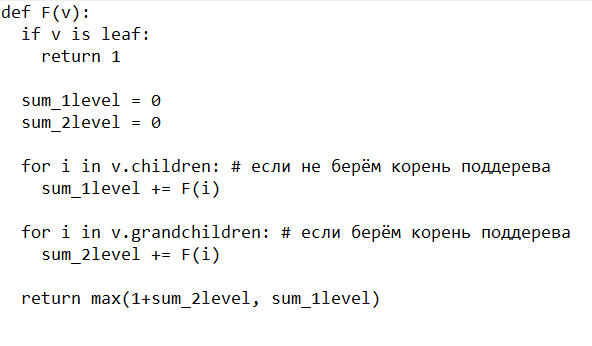
\includegraphics[width=0.7\textwidth]{code}
\end{center}

Корректнсть: докажем корректность индукцией по глубине дерева $ n $.\\
Б.И. для $ n = 1,2 $ очевидно алгоритм работает корректно.\\
Ш.И. пусть алгоритм работает корректно для глубины не больше, чем $ n $, докажем что для $ n+1 $ он тоже будет работать верно\\
По описаным в начале рассуждениям независимое множество в новом дереве глубины $ n+1 $ будет получено из максимального независимого множества глубины $ n-1 $ (которое мы находим верно по П.И.) и добавкой либо детей либо внуков каждой из вершины на $ n-1 $ уровне. Из этих вариантов алгоритм находит максимальный. Следовательно, шаг индукции доказан (рекурсивный алгоритм, мы его строим как индукцию).\\

Сложность: рассматриваем все вершины и рёбра дерева, поэтому сложность алгоритма $ O(|V|+|E|)$













\end{document} % конец документа